\section{Appendix}

\begin{frame}
    \begin{center}
        \LARGE Appendix
    \end{center}
\end{frame}



\subsection{Reservoir Computer の中のダイナミクスについて}
\begin{frame}{Reservoir Computer の構造}
    \begin{columns}[T] % [T] は列を上部で揃えるオプション
  
        \begin{column}{.5\textwidth}
            Reservoir Computer の学習の計量さについて\cite{Bollt}に倣って確認する.
            \begin{itemize}
                \item $\left\{\mathbf{x}_i\right\}_{i=1}^N \subset \mathbb{R}^{d_x}$: input data.
                \item $\mathbf{r}_i \in \mathbb{R}^{d_r}$: hidden variable. $d_r>d_x$. \begin{itemize}
                    \item $\mathbf{u}_i=\mathbf{W}^{i n} \mathbf{x}_i$. $\mathbf{W}^{i n}$ はランダムに選ばれた 重み付きの $d_r \times d_x$ 行列. 
                    \item $\mathbf{r}_{i+1}=(1-\alpha) \mathbf{r}_i+\alpha q\left(\mathbf{A r}_i+\mathbf{u}_i+\mathbf{b}\right)$. 
                    
                    $\mathbf{A}:$ ランダムに選ばれた 重み付きの $d_r \times d_r$ 行列.$\alpha:$ leaking rate (後述). $\mathbf{b}:$ offset for activation, $0$ とする.
                    
                    $q:$ activation funciton. $\tanh(\cdot)$ など.
                \end{itemize}
                \item $\mathbf{y}_{i+1}=\mathbf{W}^{\text {out }} \mathbf{r}_{i+1}$: output data.\begin{itemize}
                    \item $\mathbf{W}^{\text {out }}:$ 重み付きの $d_x \times d_r$ 行列. データに対して学習される.
                \end{itemize}
            \end{itemize}
        \end{column}
        \begin{column}{.5\textwidth}
            \begin{figure}
                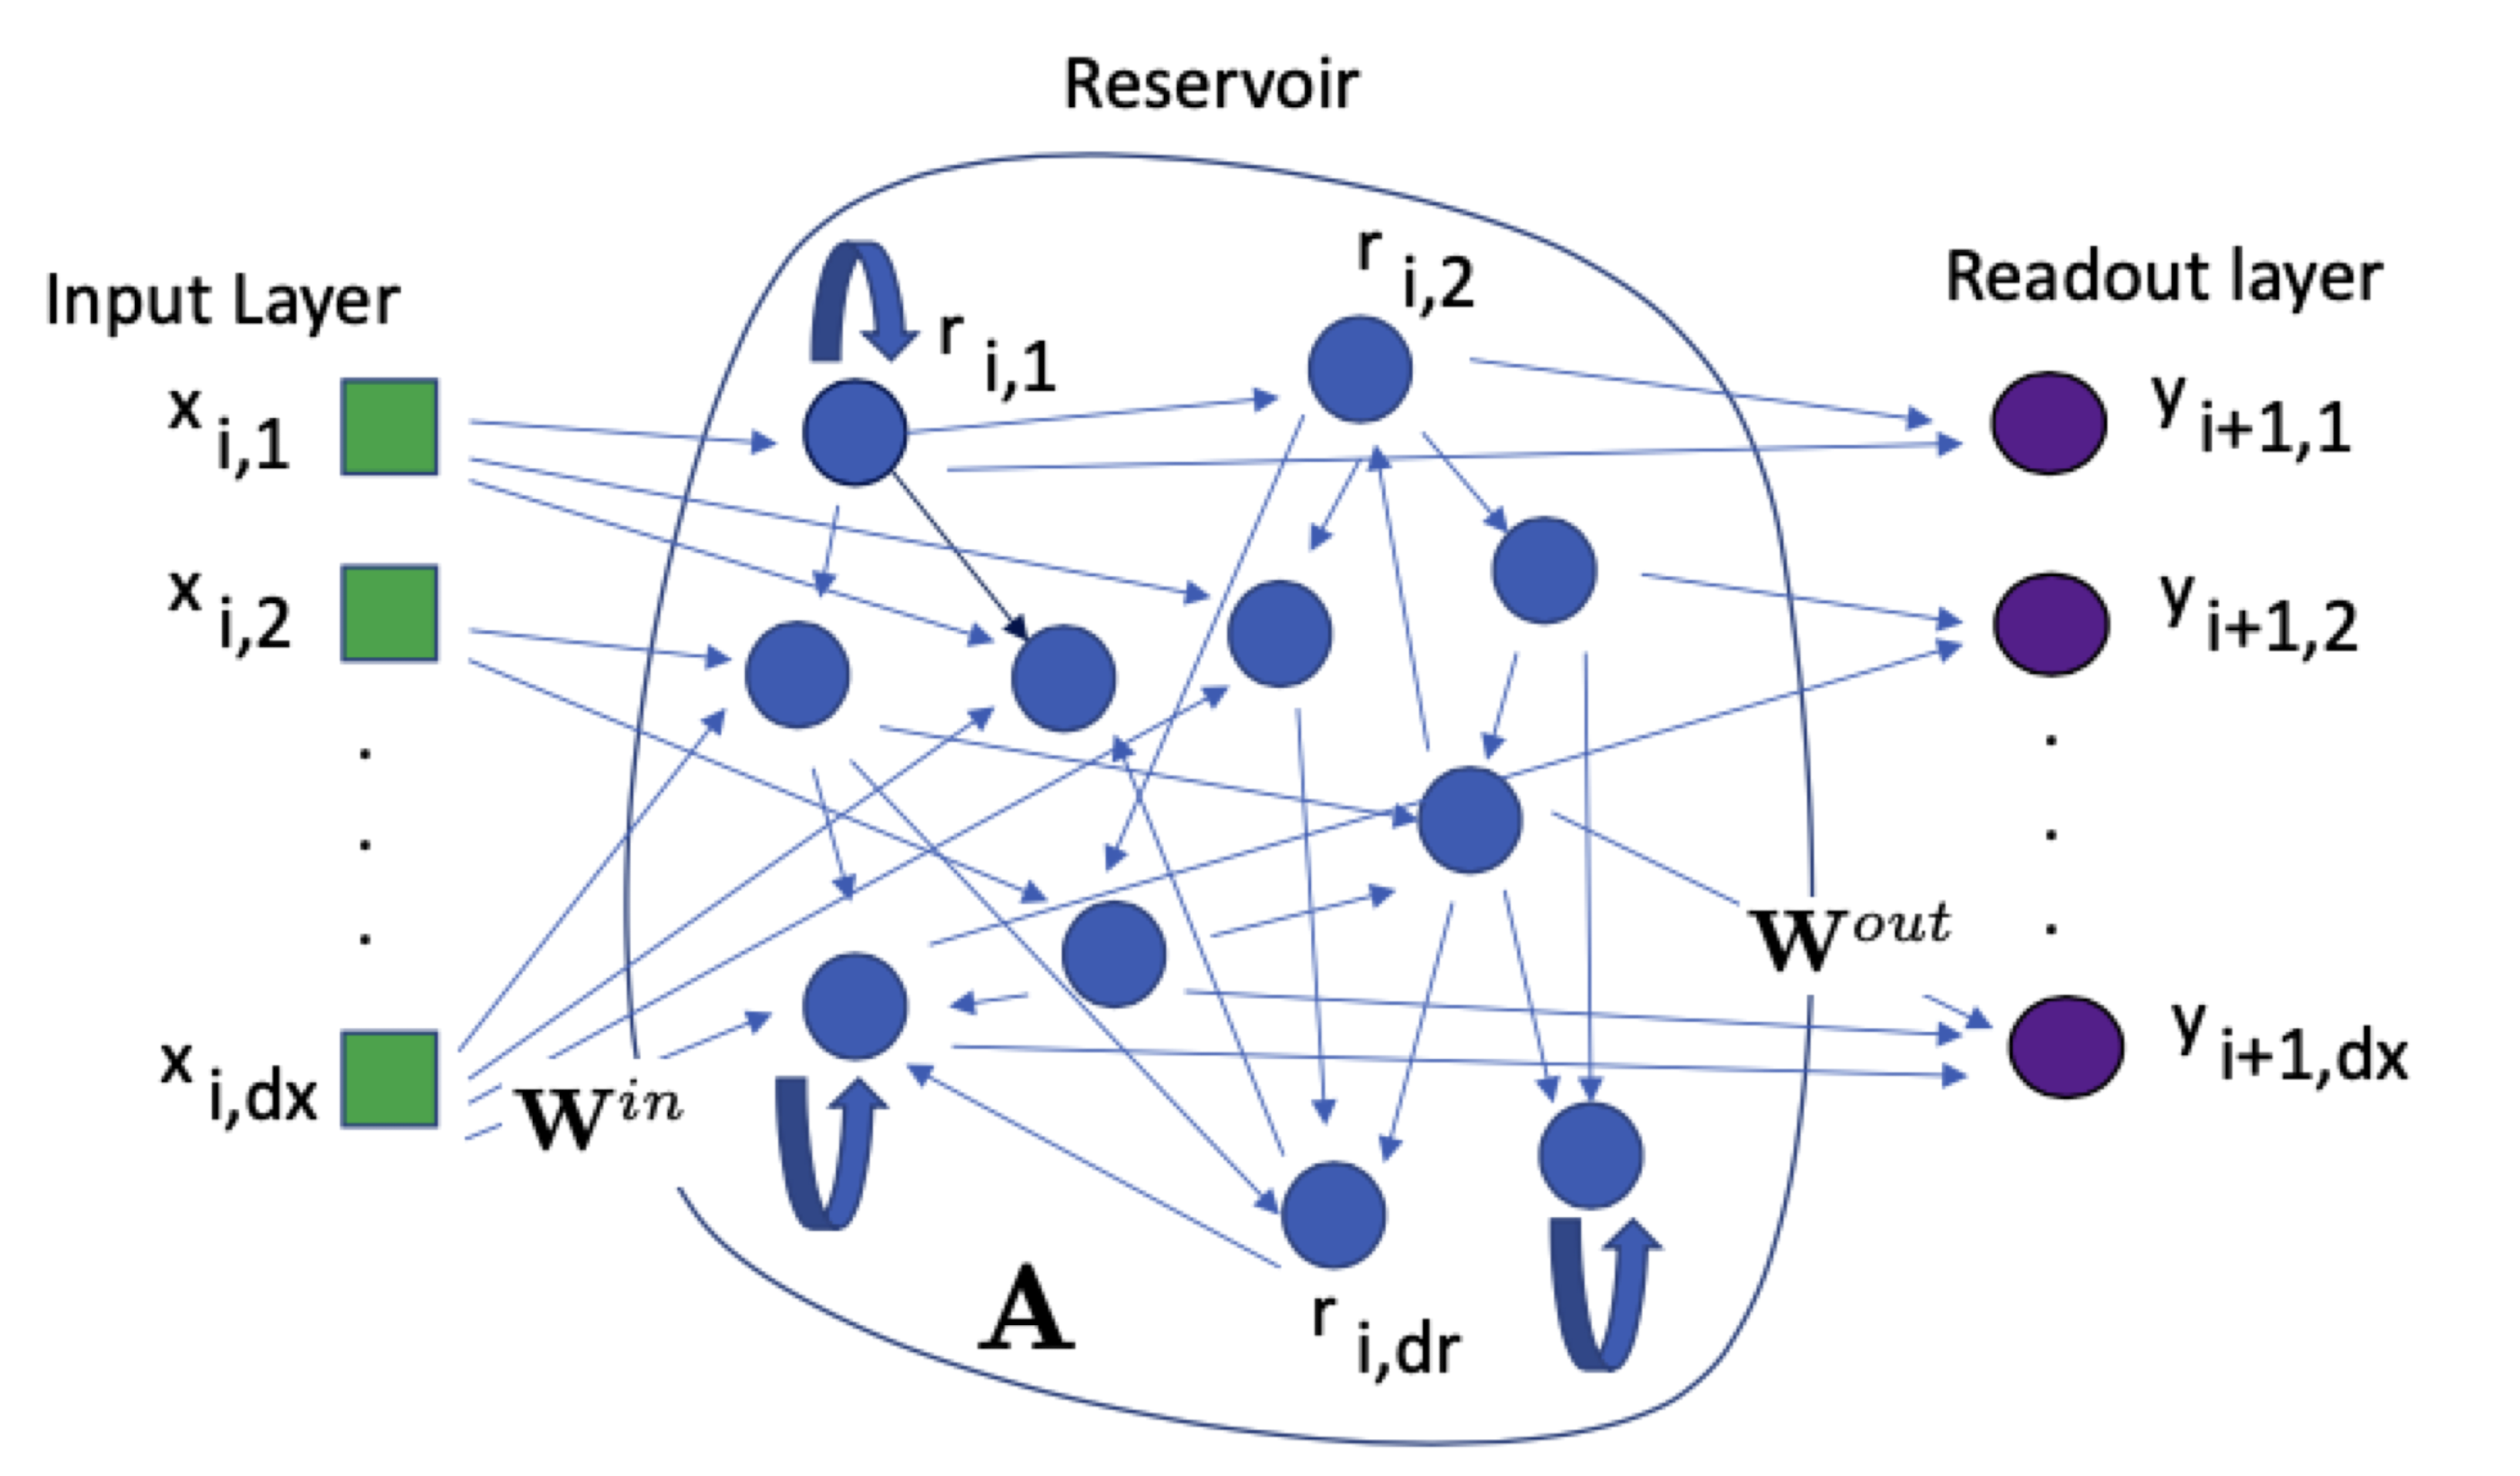
\includegraphics[width=\textwidth]{Fig/bollt_reservoir.png}
                \caption{\scriptsize{Reservoir Computer の各層の関係} \\ \tiny{Fig. 2 from \cite{Bollt}}}
            \end{figure}
        \end{column}
      \end{columns}
\end{frame}

\begin{frame}{Reservoir Computerの学習}
    \begin{itemize}
        \item Reservoir Computer の特徴は,出力層の行列 $\mathbf{W}^{\text {out }}$ のみ学習されること.\begin{itemize}
            \item 他の RNN では,$\mathbf{W}^{\text {in}}, \mathbf{A}$も学習の対象 
            
            \rightarrow 高次元空間の中で,非線形関数の $q(\cdot)$ の関わる勾配降下法最適化をしなければならない 
            
            \item Reservoir Computer はこれを回避し,$\mathbf{W}^{\text {out }}$の学習は線形な演算になる: 
            \begin{align}
                \mathbf{W}_{\text {out }}=\underset{\mathbf{V} \in \mathbb{R}^{d_x \times d_r}}{\arg \min }\|\underline{\mathbf{X}}-\mathbf{V R}\|_F=\underset{\mathbf{V} \in \mathbb{R}^{d_x \times d_r}}{\arg \min } \sum_{i=k}^N\left\|\mathbf{x}_i-\mathbf{V r}_i\right\|_2, k \geq 1 
            \end{align}
            $k > 1$ で Reservoir Computer のメモリを反映させることができる.
            \item Ridge Regression(リッジ回帰)、またはTikhonov正則化を伴う最小二乗法を用いて,過学習を防ぎながら学習させる(Hyperparameter の ridge については後述).解は形式的に次のように表される:
            \begin{align}
                \mathbf{W}^{\text {out }}:=\mathbf{X R}^T\left(\mathbf{R R}^T+\lambda \mathbf{I}\right)^{-1}
            \end{align}
        \end{itemize}
    \end{itemize}
\end{frame}

\subsection{Reservoir Computer に関する理論}
\begin{frame}
    
\end{frame}

\subsection{実験に関する先行研究}



\begin{frame}{Y. C. Lai et al. (2022) の結果 (1/2)}
    Reservior Computer は Input, Hidden, Output の三つの層から構成される.
    \begin{block}{Reservior Computer の構成:Y. C. Lai et al. (2022)}
    \vspace{0.1cm}
        \begin{minipage}{0.4\textwidth}
            \begin{figure}
                %\centering % 画像を中央揃えにする(オプション)
                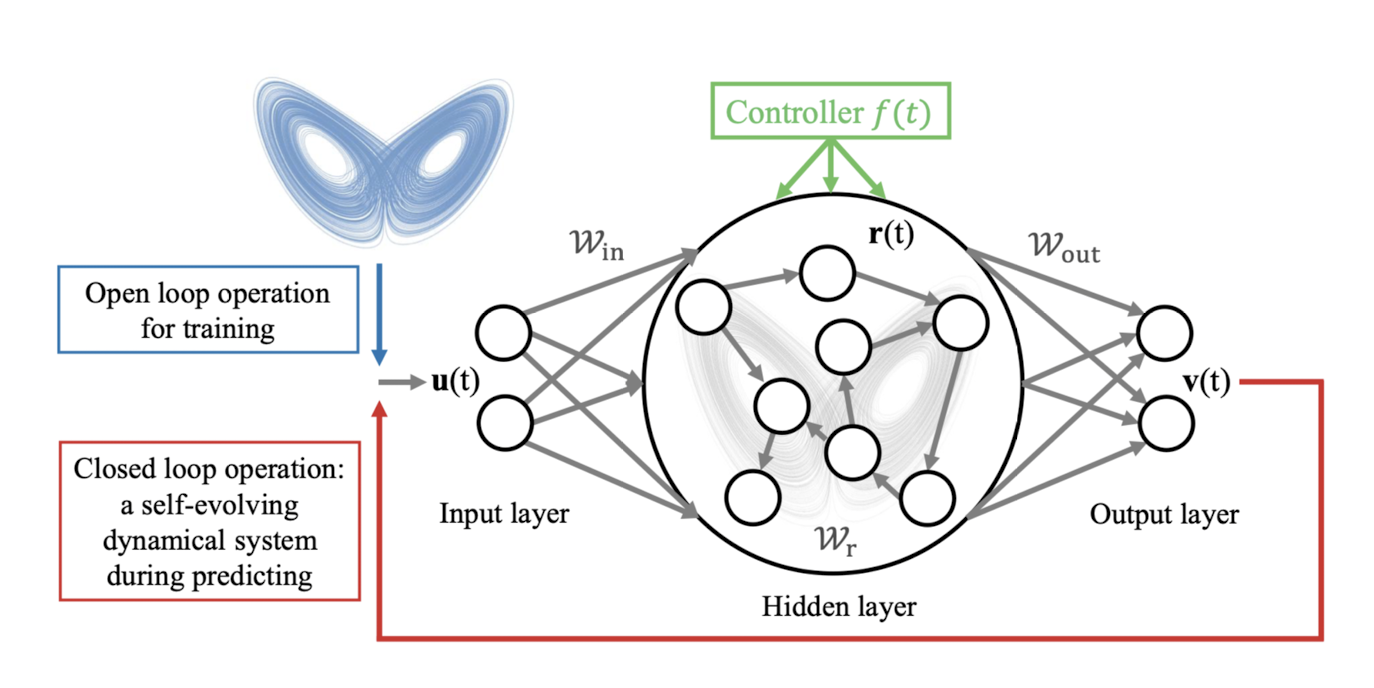
\includegraphics[width=\textwidth]{Fig/Fig.1_Lai.png}
                \caption*{Fig.1 from Y. C. Lai et al. (2022)}
                \label{Fig.1_Lai.png} % ラベルを付ける(参照する場合に使用)
            \end{figure}
        \end{minipage}%
        \begin{minipage}{0.6\textwidth}
            \begin{itemize}
                \item $\mathbf{u}(t) \in \R^{D_{\text{in}}}$: input signal. 
                \item $\mathbf{r}(t) \in \R^{D_r} $: hidden layer state vector.
                \item $f(t)$: (control) external driving signal.  
                \item $\mathcal{W}_{\text{in}} \in D_r \times D_{\text{in}}$: Weighted input matrix.  
                \item $\mathcal{W}_c$: Controller matrix.
                \item $ \mathcal{W}_r \in D_r \times D_{r}$: Weighted network matrix inside.
                \item $\mathcal{W}_{\text{out}}: D_{\text{out}} \times D_{r}$: Output weighted matrix.
            \end{itemize}
    \end{minipage}
    \end{block}
    $\mathbf{u}(t)$ に時系列モデル(low/high-dimensional Lorenz-96 climate network, driven chaotic laser systemなど),$f(t)$にはsinusoidal関数などを使用する(e.g. $f(t) = A \sin (\Omega t) + F$).
\end{frame}

\begin{frame}{Y. C. Lai et al. (2022) の結果 (2/2)}
    学習期間全体の $\mathbf{u}(t)$,全期間の $\mathbf{v}(t)$ を記録する行列をそれぞれ $\mathcal{R'}, \mathcal{V}$ とする.
    \begin{itemize}
        \item $\mathcal{W}_{\text {in }}, \mathcal{W}_c, \mathcal{W}_r$ は Reservior の学習に前もってランダムに定められる.
        \item 学習期間において,$\mathbf{u(t)}$ と $f(t)$ の実データが入力される.
        学習期間の後のself-evolving 期間では,Reservior による出力 $\mathbf{v}(t)$ と $f(t)$ の実データが予測の入力に用いられる.
        \begin{itemize}
            \item $\mathbf{r}(t)$ は 学習期間,self-evolving 期間においてそれぞれ次の式で決定される.
            \vspace{-.2cm}
            \begin{align}
                \mathbf{r}(t+\Delta t) & =(1-\alpha) \mathbf{r}(t) + \alpha \tanh \left[\mathcal{W}_r \mathbf{r}(t)+\mathcal{W}_{\text {in }} \mathbf{u}(t)+\mathcal{W}_c f(t)\right] \label{Lai_r1}\\
                \mathbf{r}(t+\Delta t) & =(1-\alpha) \mathbf{r}(t) + \alpha \tanh \left[\mathcal{W}_r \mathbf{r}(t)+\mathcal{W}_{\text {in }} \mathcal{W}_{\text {out }} \mathbf{r}^{\prime}(t)+\mathcal{W}_c f(t)\right]\label{Lai_r2}
            \end{align}
        \end{itemize}
        \item 複数の $f(t)$ に対して Reservior を sequential に学習させることで,未知の外力がある場合でも予測できるようにする.また,Hyperparameter に関する最適化を行う(後述).
        \item Reservoir に次式における$\mathcal{V}, \mathcal{R'}$ 間のLinear Regressionを通じて$\mathcal{W}_{\text {out }}$ を学習させる.
        \vspace{-.2cm}
        \begin{align}
            \mathcal{W}_{\text {out }}=\mathcal{V} \cdot \mathcal{R}^{\prime T}\left(\mathcal{R}^{\prime} \cdot \mathcal{R}^{\prime T}+\beta \mathcal{I}\right)^{-1}
        \end{align}
    \end{itemize}

\end{frame}


\subsection{Hyperparameters の最適化}
\begin{frame}{Reservoir に関する Hyperparameters}
    Reservoir に関する Hyperparameter のうち,最適化の対象としたものを記した.説明は,\cite{rpy_doc}の Tutorial 4 を参考にした.
    \begin{enumerate}
        \item Cell Number (N): セル数.
        \item spectral radius (sr): スペクトル半径.Reservoir の 行列 $\mathcal{W}$ の固有値の絶対値の最大値.\begin{itemize}
            \item 小さいと安定したダイナミクス、大きいとカオス的なダイナミクス.
            \item 理論的には$1$ に近いと Reservoir の初期条件に影響を受けにくく,良好な memory を持つことが推測される.
        \end{itemize}
        \item input scaling (iss): Reservoir の入力 $\mathcal{W}_{in}$ に適用される係数.入力にゲインを加える.\begin{itemize}
            \item 高くするとReservoir と 入力の相関を(飽和点まで)高める.
            \item 低くすると Reservoir は外部の入力より自身のダイナミクスに強く影響を受ける.
            \item 多変量時系列データの各変数の影響度を調整可能.
        \end{itemize}
        \item leaking rate (lr): 次ステップの決定に際しての現在の状態と新しい入力の影響度の割合.\begin{itemize}
            \item 高い(低い)と惰性が高く(低く),過去の記憶状態が高く(低く)なる.
            \item ESN のネットワークがその状態を変化させる速度を制御する.
        \end{itemize}
        \item ridge (ridge): 
    \end{enumerate}
\end{frame}

\begin{frame}{Hyperparameters 最適化のアルゴリズム}
    Hyperparameters の最適化には python ライブラリである Optuna を用いた.
     
    Optunaで実装されている Hyperparameters の最適化アルゴリズムは例えば以下がある.
    \begin{columns}[T] % [T] は列を上部で揃えるオプション
        \begin{column}{.5\textwidth}
            

            \begin{block}{optuna.samplers: from \cite{optuna_doc}}
                \begin{enumerate}
                    \item \textbf{optuna.samplers.RandomSampler}: ランダムサンプリングを使用するサンプラー。
                    \item \textbf{optuna.samplers.TPESampler}: TPE(Tree-structured Parzen Estimator)アルゴリズムを使用するサンプラー。
                    \item \textbf{optuna.samplers.CmaEsSampler}: CMA-ES(Covariance Matrix Adaptation Evolution Strategy)をバックエンドとして使用するサンプラー。
                \end{enumerate}
                
            \end{block}
        
        \end{column}
        \begin{column}{.5\textwidth}
            \begin{itemize}
                \item この研究では,CmaEsSampler (最終的に採用), TPESampler と hyperopt という別のpython ライブラリの random search を用いた.\begin{itemize}
                    \item 経験的に,同順により好ましい best value を与えた.
                    
                \end{itemize}
                \item また,Optuna搭載の pruner も利用した.\begin{itemize}
                    \item 見込みの悪い Hyperparameters のセットを見限ること.
                    \item 使用したのは SuccessiveHalvingPruner.
                \end{itemize}
                \item なお,hyperopt には Optunaのいくつかの機能は搭載されていないので注意.
            \end{itemize}
        \end{column}
      \end{columns}


\end{frame}


\subsection{実験のパラメータ設定}

\begin{frame}
    \begin{columns}[T] % [T] は列を上部で揃えるオプション
        \begin{column}{.5\textwidth}
            \begin{itemize}
                \item Rössler系の数値シミュレーション\begin{itemize}
                    \item $A = 1.0$ 
                    \item $a = 0.2,\ b = 0.2,\ c = 5.7.$ 
                    \item 初期条件:$\left[ X_0, Y_0, Z_0 \right] = [1.0, 1.0, 1.0]$ 
                    \item 時間範囲:$t_\text{span} = [0, 4510].$ 
                    \item 位相シフト時間:$p = 8$ に対して Hyperparameter を最適化. 
                    \item 注.配列データは $1$ タイムステップに対して $10$ 個データポイントをとって生成したので,長さ $[0, 45100]$ である.
                \end{itemize}
                \item Optunaの最適化
                \begin{itemize}
                    \item $\text{nb seeds} = 3$
                    \item $\text{nb trials} = 3000$ 
                    \item 最適化アルゴリズム:CmaEsSampler
                    \item pruner: SuccessiveHalvingPruner
                    \item $\text{train len} = 20000$
                    \item $\text{test len} = 10000$
                \end{itemize}
            \end{itemize}
        \end{column}
        \begin{column}{.5\textwidth}
            \begin{itemize}
                \item Hyperparameters の探索空間\begin{itemize}
                    \item N = 10000: 固定

                    sr:  (1e-2, 10, log = True)

                    lr: (1e-3, 1, log = True)

                    iss: (0, 1)
                    
                    ridge: (1e-9, 1e-2, log = True)

                    \item 一様ランダムにサンプリング.
                    \item log = True で$\log$ をとって一様ランダムにサンプリング.
                \end{itemize}
                \item 採用した Hyperparameters のセット\begin{itemize}
                    \item Best value: 0.0017332259260817507
                    Best parameters: {
                        
                        'sr': 0.568437354122632, 
                        
                        'lr': 0.33989147591891816, 
                        
                        'iss': 0.08827385538440446, 
                        
                        'ridge': 1.30084237042553e-08}
                \end{itemize}
            \end{itemize}
        \end{column}
      \end{columns}
    
\end{frame}

\subsection{結果のまとめ}
\begin{frame}{self-evolve 期間における予測結果:位相シフトが$8, 10$のとき(再掲)}
    \begin{columns}[T] % [T] は列を上部で揃えるオプション
      \begin{column}{.5\textwidth}
        \begin{figure}
          \vspace{-.5cm}
          % 画像1
          \begin{minipage}[c][.27\textheight][c]{\linewidth}
            \centering
            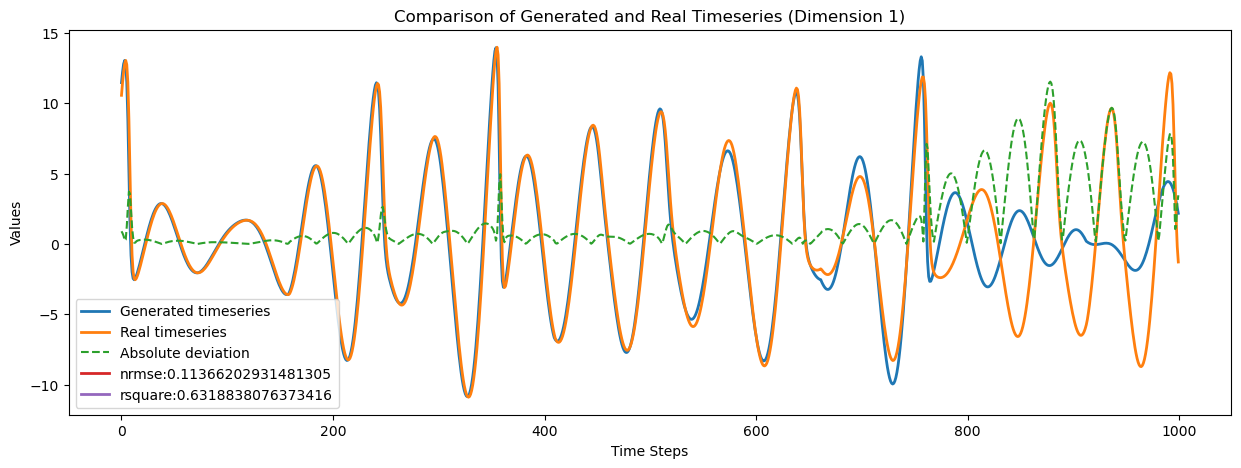
\includegraphics[width=0.7\linewidth]{Fig/8.x.png}
          \end{minipage}
      
          \vspace{-.5em}
  
          % 画像2
          \begin{minipage}[c][.27\textheight][c]{\linewidth}
            \centering
            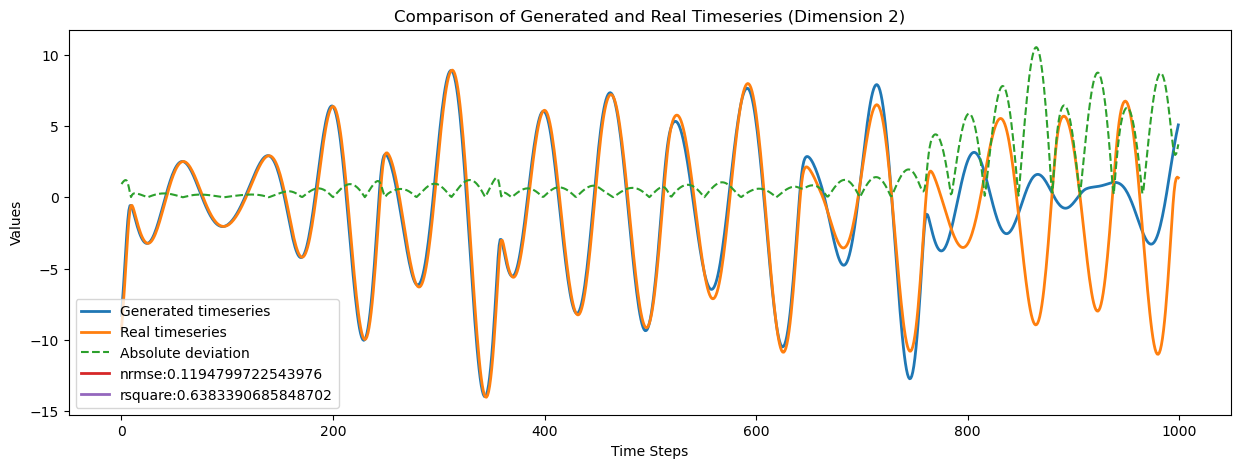
\includegraphics[width=0.7\linewidth]{Fig/8.y.png}
          \end{minipage}
          
          \vspace{.5em}
          % 画像3
          \begin{minipage}[c][.27\textheight][c]{\linewidth}
            \centering
            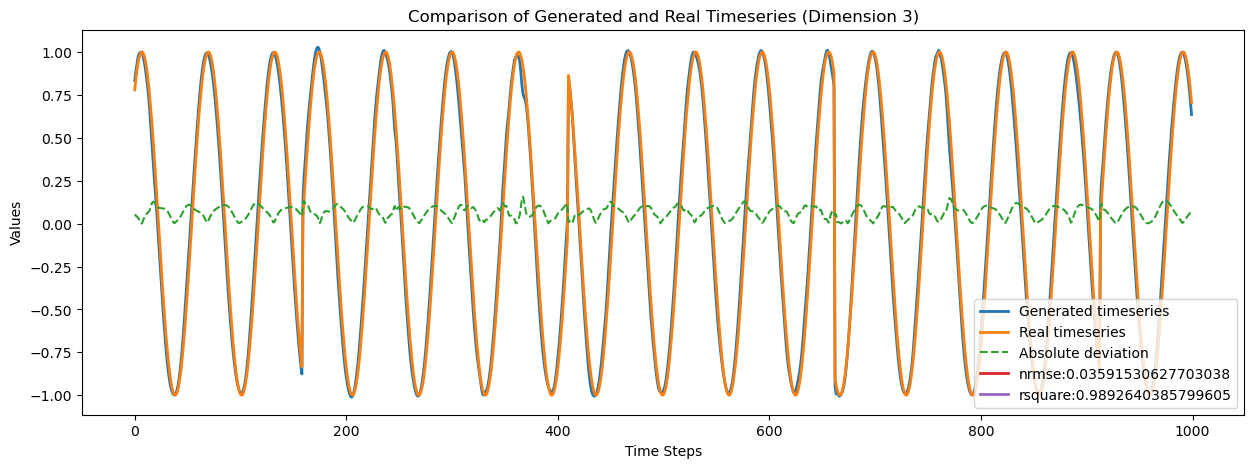
\includegraphics[width=0.7\linewidth]{Fig/8.p.png}
            \caption{\scriptsize{位相シフト(8時間分)のある外力付きRösslerモデルの予測.上から $x, y, P(t)$. }}
          \end{minipage}
        \end{figure}
      \end{column}
      \begin{column}{.5\textwidth}
        \begin{figure}
          \vspace{-.5cm}
          % 画像1
          \begin{minipage}[c][.27\textheight][c]{\linewidth}
            \centering
            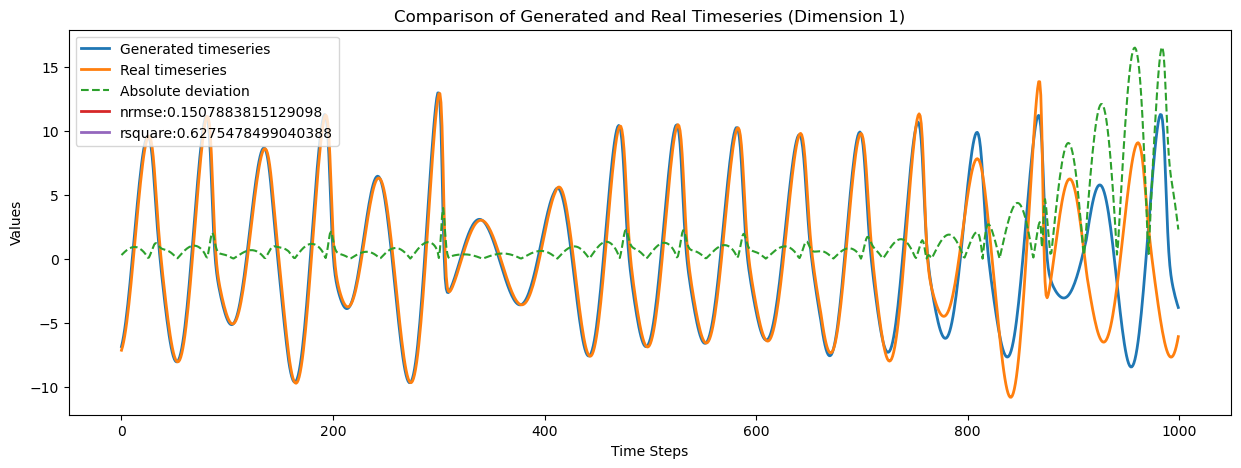
\includegraphics[width=0.7\linewidth]{Fig/10.x.png}
          \end{minipage}
      
          \vspace{-.5em}
  
          % 画像2
          \begin{minipage}[c][.27\textheight][c]{\linewidth}
            \centering
            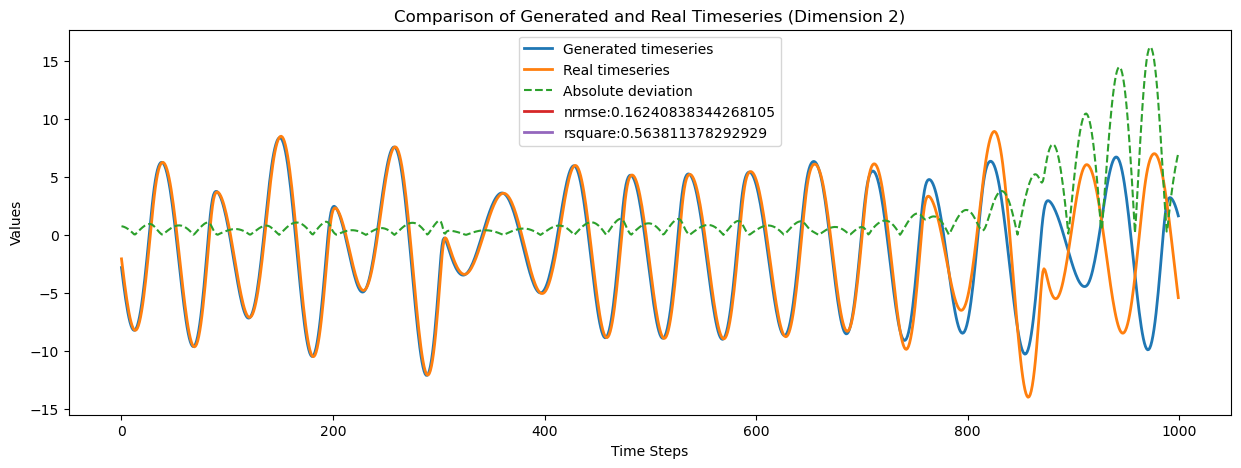
\includegraphics[width=0.7\linewidth]{Fig/10.y.png}
          \end{minipage}
          
          \vspace{.5em}
          % 画像3
          \begin{minipage}[c][.27\textheight][c]{\linewidth}
            \centering
            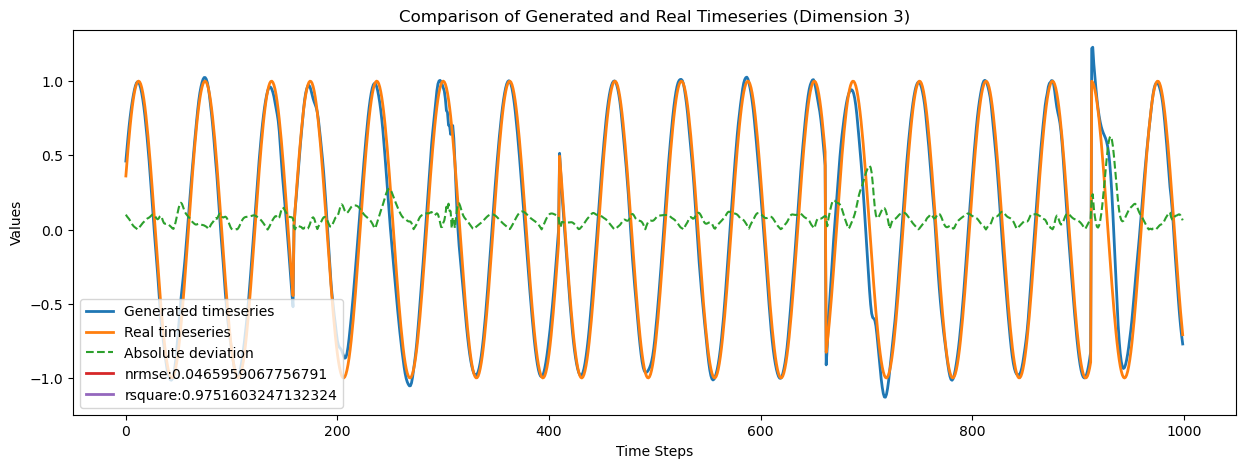
\includegraphics[width=0.7\linewidth]{Fig/10.p.png}
            \caption{\scriptsize{位相シフト(10時間分)のある外力付きRösslerモデルの予測.上から $x, y, P(t)$.}}
          \end{minipage}
        \end{figure}
      \end{column}
    \end{columns}
  \end{frame}

  \begin{frame}{self-evolve 期間における予測結果:位相シフトが$4, 6$のとき}
  \begin{columns}[T] % [T] は列を上部で揃えるオプション
    \begin{column}{.5\textwidth}
        \begin{figure}
            \vspace{-.5cm}
            % 画像1
            \begin{minipage}[c][.27\textheight][c]{\linewidth}
              \centering
              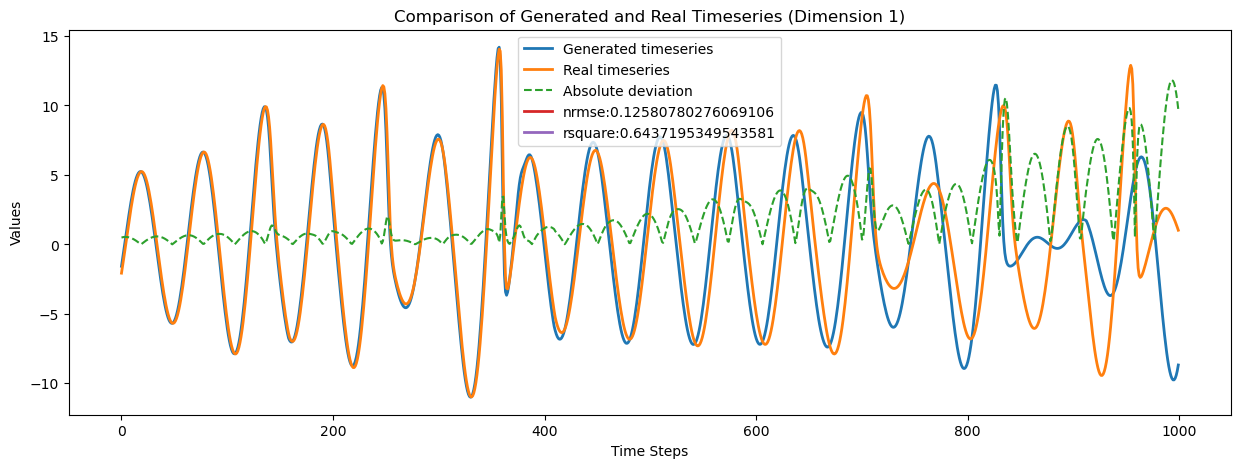
\includegraphics[width=0.7\linewidth]{Fig/4.x.png}
            \end{minipage}
        
            \vspace{-.5em}
    
            % 画像2
            \begin{minipage}[c][.27\textheight][c]{\linewidth}
              \centering
              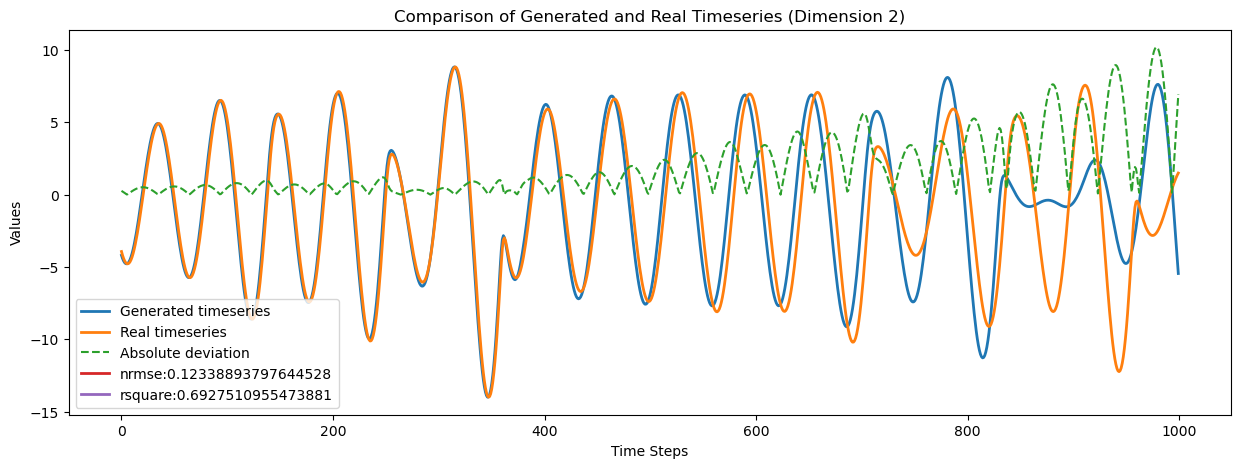
\includegraphics[width=0.7\linewidth]{Fig/4.y.png}
            \end{minipage}
            
            \vspace{.5em}
            % 画像3
            \begin{minipage}[c][.27\textheight][c]{\linewidth}
              \centering
              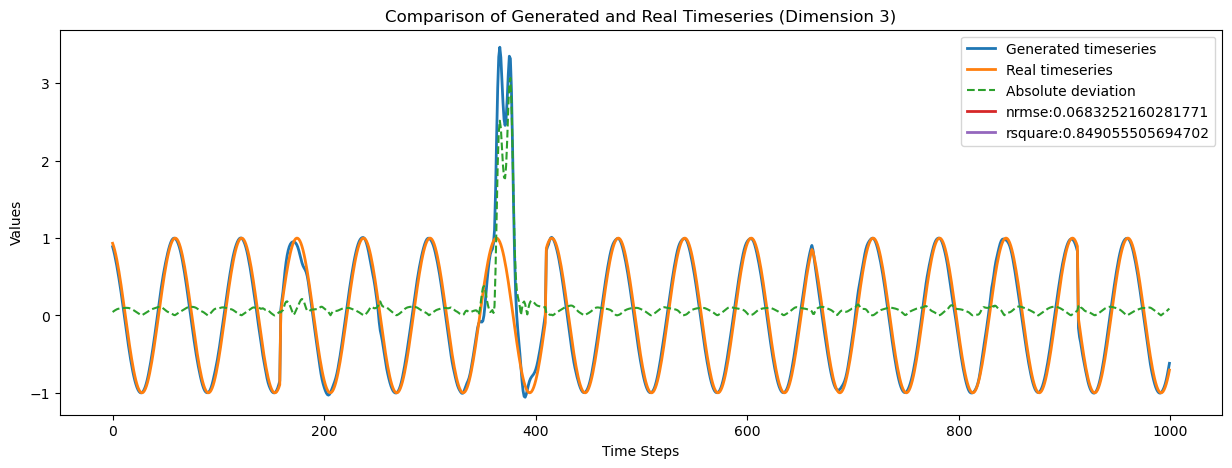
\includegraphics[width=0.7\linewidth]{Fig/4.p.png}
              \caption{\scriptsize{位相シフト(4時間分)のある外力付きRösslerモデルの予測.上から $x, y, P(t)$. }}
            \end{minipage}
          \end{figure}

    \end{column}
    \begin{column}{.5\textwidth}
      \begin{figure}
        \vspace{-.5cm}
        % 画像1
        \begin{minipage}[c][.27\textheight][c]{\linewidth}
          \centering
          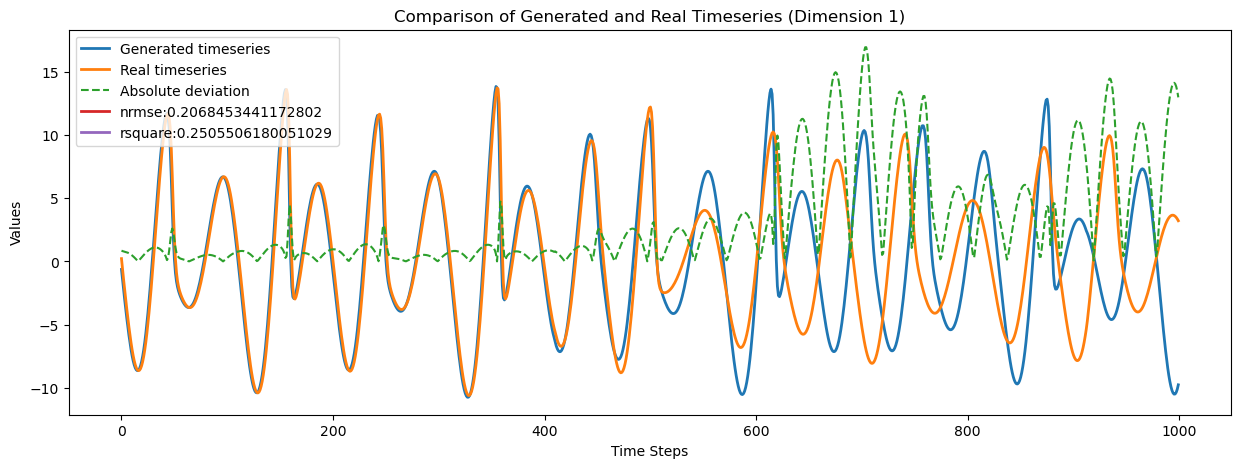
\includegraphics[width=0.7\linewidth]{Fig/6.x.png}
        \end{minipage}
    
        \vspace{-.5em}

        % 画像2
        \begin{minipage}[c][.27\textheight][c]{\linewidth}
          \centering
          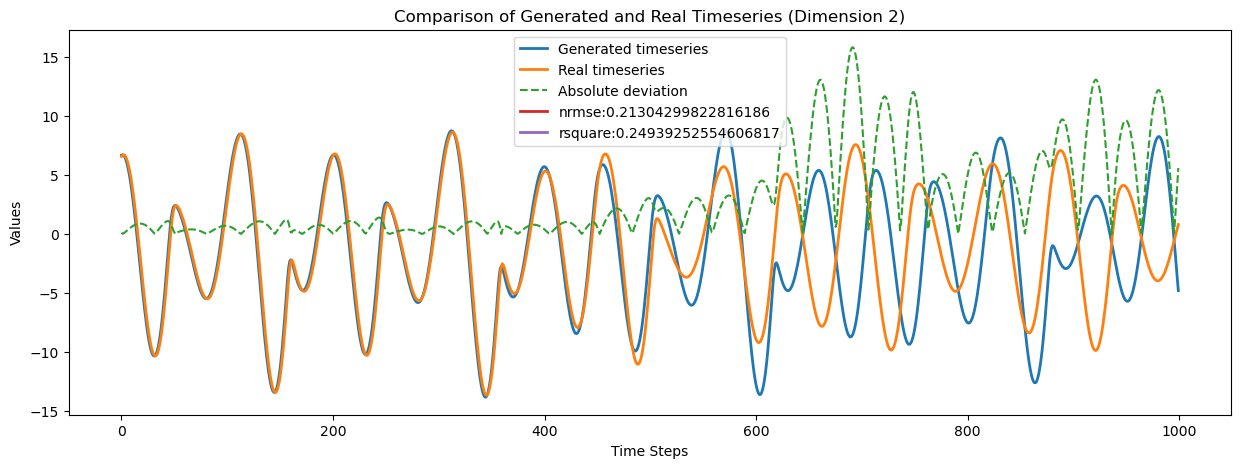
\includegraphics[width=0.7\linewidth]{Fig/6.y.png}
        \end{minipage}
        
        \vspace{.5em}
        % 画像3
        \begin{minipage}[c][.27\textheight][c]{\linewidth}
          \centering
          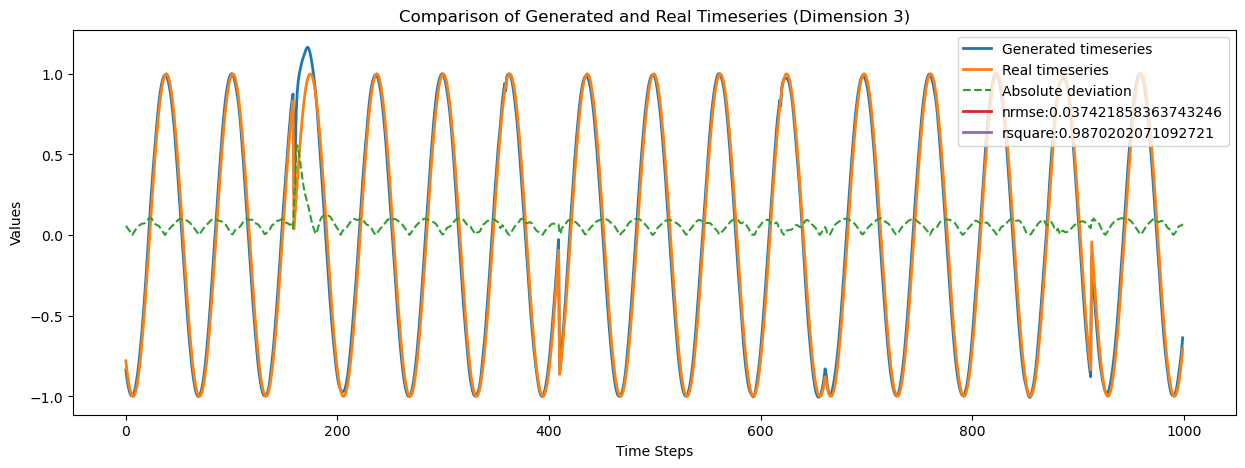
\includegraphics[width=0.7\linewidth]{Fig/6.p.png}
          \caption{\scriptsize{位相シフト(6時間分)のある外力付きRösslerモデルの予測.上から $x, y, P(t)$.}}
        \end{minipage}
      \end{figure}
    \end{column}
  \end{columns}
\end{frame}

\begin{frame}{self-evolve 期間における予測結果:位相シフトが$-4, -8$のとき}
    \begin{columns}[T] % [T] は列を上部で揃えるオプション
      \begin{column}{.5\textwidth}
        \begin{figure}
            \vspace{-.5cm}
            % 画像1
            \begin{minipage}[c][.27\textheight][c]{\linewidth}
              \centering
              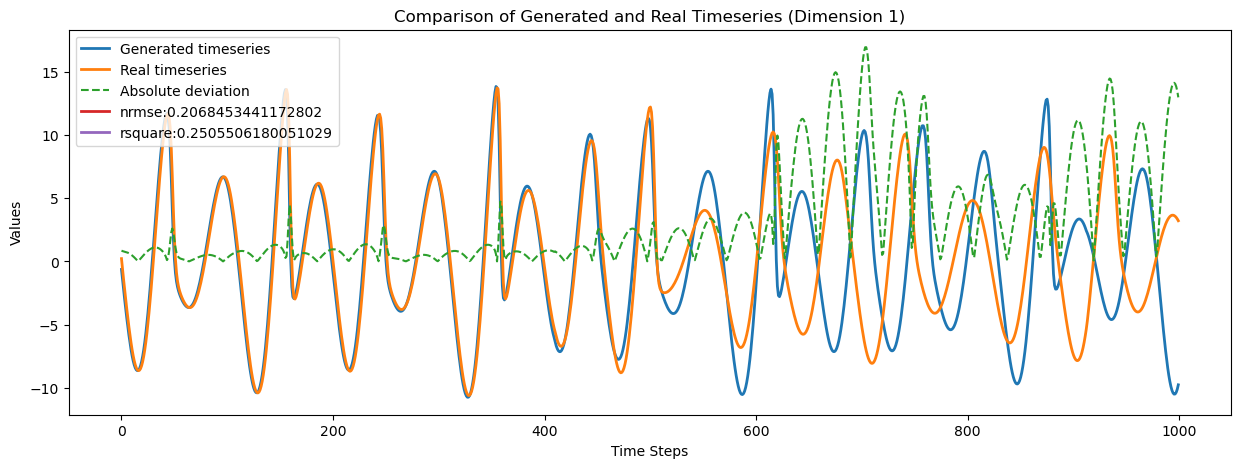
\includegraphics[width=0.7\linewidth]{Fig/-4.x.png}
            \end{minipage}
        
            \vspace{-.5em}
    
            % 画像2
            \begin{minipage}[c][.27\textheight][c]{\linewidth}
              \centering
              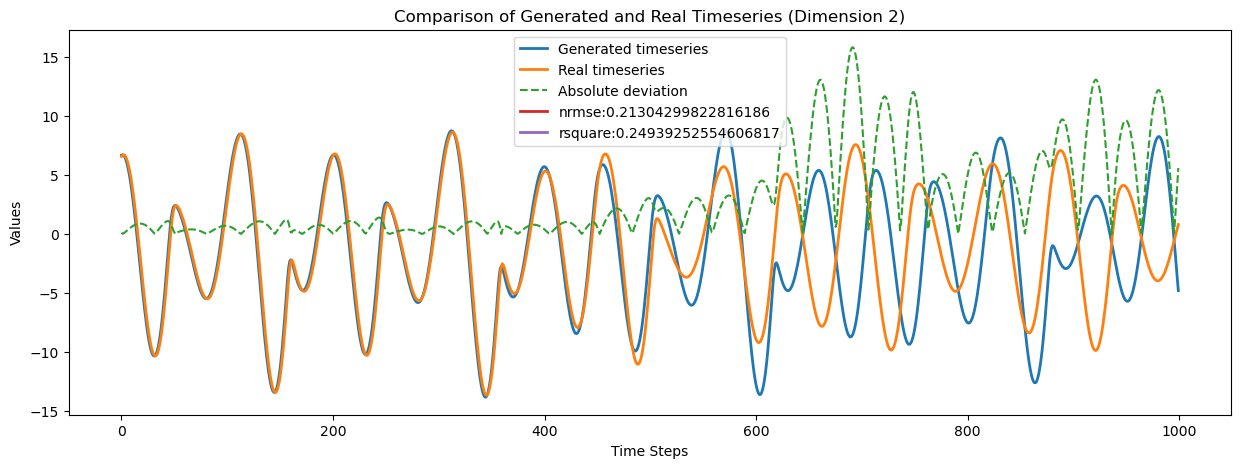
\includegraphics[width=0.7\linewidth]{Fig/-4.y.png}
            \end{minipage}
            
            \vspace{.5em}
            % 画像3
            \begin{minipage}[c][.27\textheight][c]{\linewidth}
              \centering
              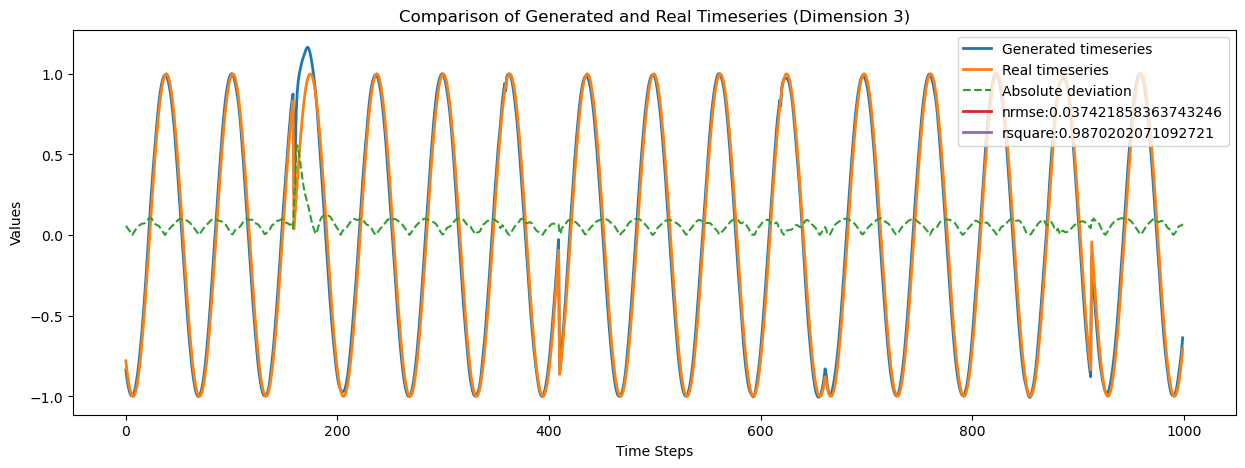
\includegraphics[width=0.7\linewidth]{Fig/-4.p.png}
              \caption{\scriptsize{位相シフト(-4時間分)のある外力付きRösslerモデルの予測.上から $x, y, P(t)$. }}
            \end{minipage}
          \end{figure}
      \end{column}
      \begin{column}{.5\textwidth}
        \begin{figure}
          \vspace{-.5cm}
          % 画像1
          \begin{minipage}[c][.27\textheight][c]{\linewidth}
            \centering
            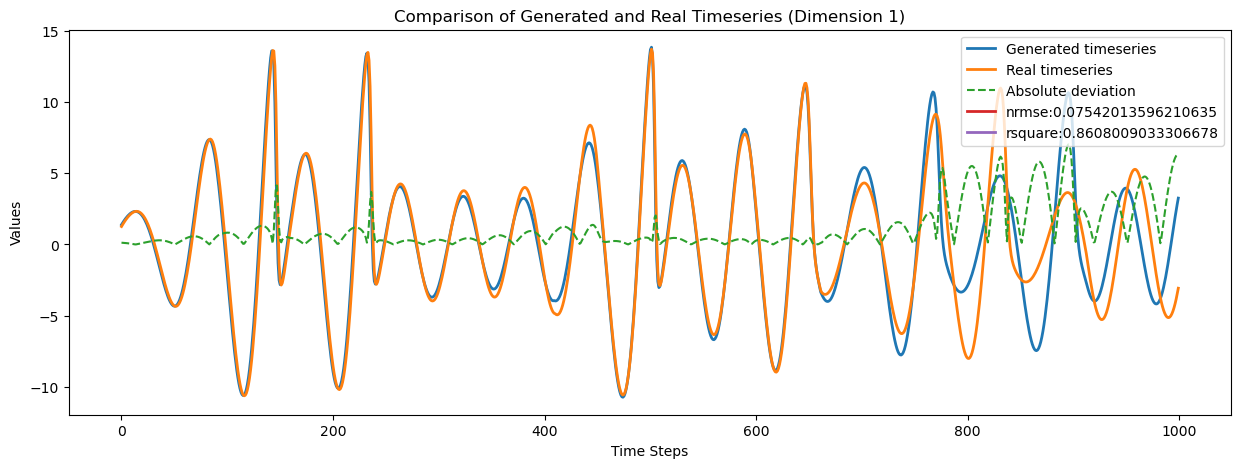
\includegraphics[width=0.7\linewidth]{Fig/-8.x.png}
          \end{minipage}
      
          \vspace{-.5em}
  
          % 画像2
          \begin{minipage}[c][.27\textheight][c]{\linewidth}
            \centering
            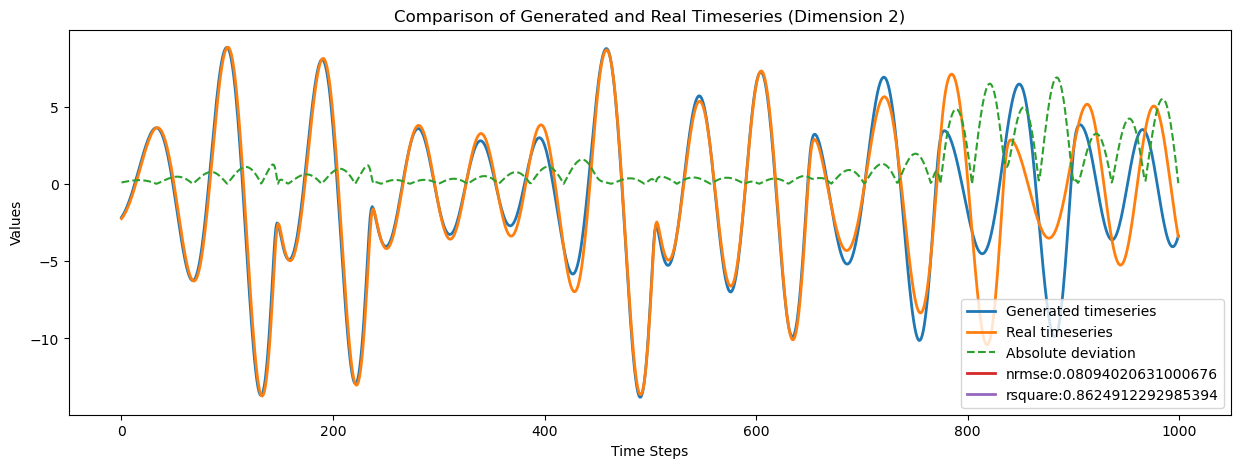
\includegraphics[width=0.7\linewidth]{Fig/-8.y.png}
          \end{minipage}
          
          \vspace{.5em}
          % 画像3
          \begin{minipage}[c][.27\textheight][c]{\linewidth}
            \centering
            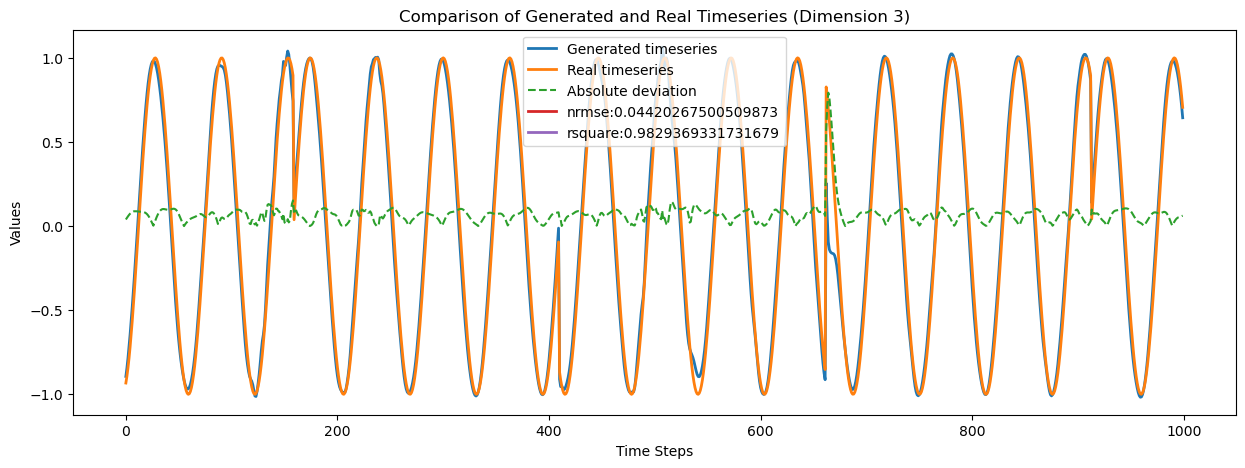
\includegraphics[width=0.7\linewidth]{Fig/-8.p.png}
            \caption{\scriptsize{位相シフト(-8時間分)のある外力付きRösslerモデルの予測.上から $x, y, P(t)$.}}
          \end{minipage}
        \end{figure}
      \end{column}
    \end{columns}
  \end{frame}
  
  



\section{参考文献}

\begin{frame}{参考文献 - 1}
    \begin{thebibliography}{99}    
        \bibitem[1]{Bollt}
        Bollt, E.M. (2020). On explaining the surprising success of reservoir computing forecaster of chaos? The universal machine learning dynamical system with contrast to VAR and DMD. Chaos, 31 1, 013108 .

        \bibitem[2]{Trouvain}
        Trouvain, N., Pedrelli, L., Dinh, T. T., Hinaut, X. (2020) Reservoirpy: an efficient and user-friendly library to design echo state networks. In International Conference on Artificial Neural Networks (pp. 494-505). Springer, Cham.

        \bibitem[3]{Yamaguchi et al.}
        Yamaguchi, Y., Suzuki, T., Mizoro, Y., Kori, H., Okada, K., Chen, Y., Fustin, J. M., Yamazaki, F., Mizuguchi, N., Zhang, J., Dong, X., Tsujimoto, G., Okuno, Y., Doi, M., and Okamura, H. (2013). Mice genetically deficient in vasopressin V1a and V1b receptors are resistant to jet lag. Science (New York, N.Y.), 342(6154), 85–90. 
    \end{thebibliography}
\end{frame}

\begin{frame}{参考文献 - 2}
    \begin{thebibliography}{99}    
        \bibitem[4]{optuna_doc}
        Optuna. (2018). Optuna Documentation. Retrieved from \url{https://optuna.readthedocs.io/en/stable/} [Accessed on: \today]

        \bibitem[5]{rpy_doc}
        ReservoirPy Team. (2020). ReservoirPy Documentation. Retrieved from \url{https://reservoirpy.readthedocs.io/en/latest/} [Accessed on: \today].

    \end{thebibliography}
\end{frame}
